\chapter{Fundamentals}
This chapter introduces the fundamental concepts necessary for the research.
\section{Surface path-tracing}
We aim to implement a physically based renderer in order to validate the results of our research.
The key property of physically based approaches is the conservation of energy which is given by the rendering equation \cite[p. 1]{rendering_equation}:
\begin{equation}
    \label{eq:render_equation}
    L(\boldsymbol{x}, \omega_o) = L_e(\boldsymbol{x}, \omega_o) + \int_{\mathcal{S}^2} f(\boldsymbol{x}, \omega_o, \omega_i) L(\boldsymbol{y}, -\omega_i) |n_x \cdot w_i| d\omega_i.
\end{equation}
It states that the radiance at a point $x$ in direction $\omega_o$ is given by the emitted radiance at this point plus the integral over the unit sphere $\mathcal{S}^2$ of the \ac{brdf} $f$ times the radiance $L$ coming from $\omega_i$ times the absolute value between the normal $n_x$ at point $x$ and the incident direction $\omega_i$.
Since this equation is in general not analytically solvable we can use Monte Carlo integration to solve it numerically.
For that we have to replace the integral by a sum and divide each summand by the number of summands and by the probability of sampling a direction $\omega_i$ \cite[p. 856]{pbr}:
\begin{equation}
    L(\boldsymbol{x}, \omega_o) = L_e(\boldsymbol{x}, \omega_o) + \frac{1}{N}\sum_{i=1}^{N} \frac{f(\boldsymbol{x}, \omega_o, \omega_i) L(\boldsymbol{y}, -\omega_i) |n_x \cdot w_i|}{p(\omega_i)}.
\end{equation}
The recursive nature of this equation can be observed immediately as we could substitute the radiance $L$ in the sum by the whole equation.
However an implementation in this way is infeasible since that would lead to an exponential growth in the compute time and memory consumption with the recursion depth.
As a solution to this problem \citeauthor{rendering_equation} proposed the \textit{path-tracing} algorithm \cite[p. 6]{rendering_equation}.
Instead of sampling $N$ new directions at each point of intersecting the geometry, we sample a single direction at each intersection point starting at the camera until we hit a light source \cite[p. 6]{rendering_equation}.
This gives us the \textit{path}.
When we repeat this process a large number of times we still get the same result as with using the recursive approach \cite[p. 870]{pbr}.

\section{Volumetric path-tracing}
Since we want to represent our \acsp{lod} by volumes the following chapter introduces how path-tracing can be extended to volumes.
\subsection{Theory of Light Propagation in Participating Media}
\label{subsec:theory_of_light_propagation_in_participating_media}
For volumes the radiance along a ray is determined by the in- and out-scattering as well as the emission and absorption properties of the medium \cite[p. 3]{novak_overview}.
\begin{figure}[!ht]
    \centering
    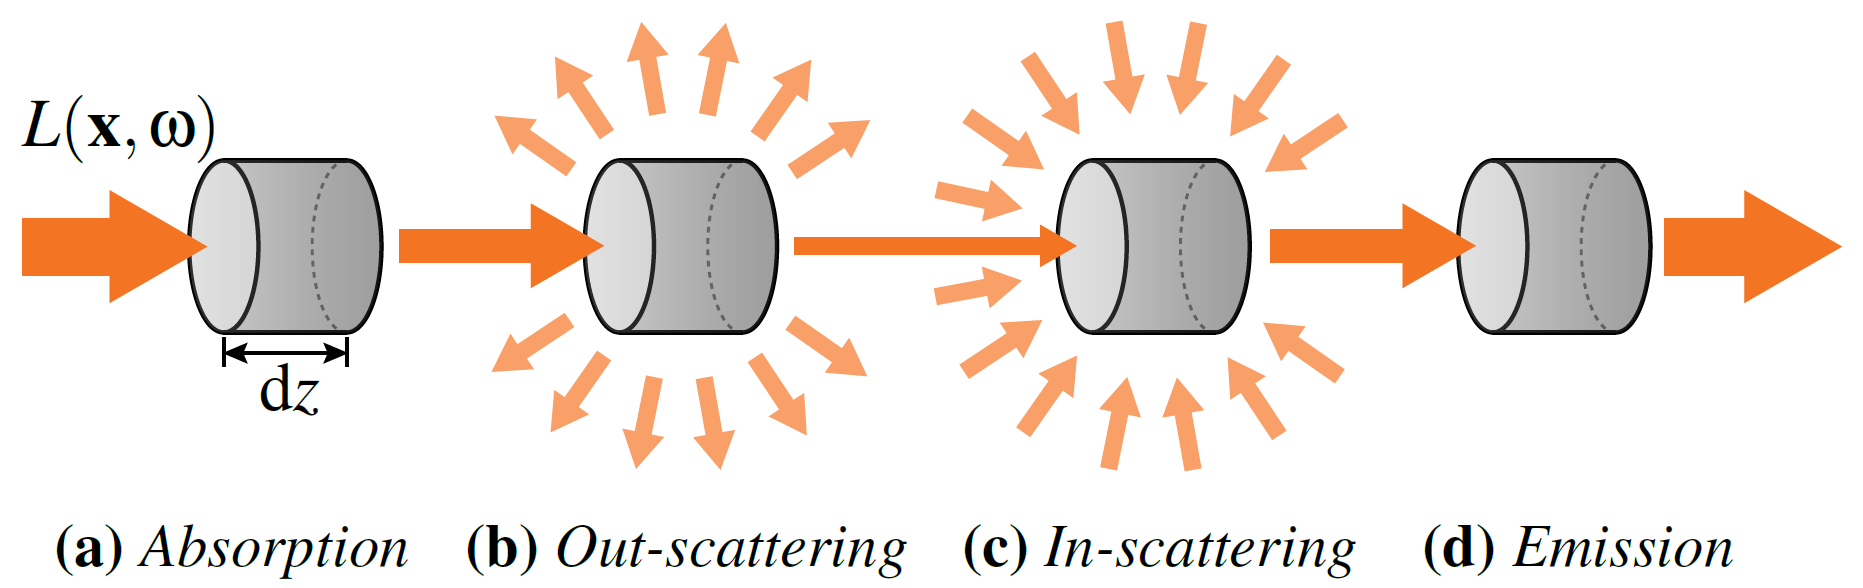
\includegraphics[width=0.8\linewidth]{img/novak_volume_effects.png}
    \caption{The physical effects that are modeled by the \textit{radiative transfer equation} (Image from \cite[p. 2]{novak_overview}).}
    \label{fig:novak_volume_effects}
\end{figure}
The \textit{scattering coefficient} $\mu_s$ and the \textit{absorption coefficient} $\mu_a$ quantify these effects \cite[p. 2]{novak_overview}.
The sum of $\mu_s$ and $\mu_a$ is called the \textit{extinction coefficient} $\mu_t=\mu_a + \mu_s$ and accounts for either of the effects \cite[p. 2]{novak_overview}.
With the integral form of the \textit{radiative transfer equation} we have a way to formalize the scattering, emission and absoption of the medium \cite[p. 3]{novak_overview}:
\begin{equation}
    \label{eq:radiative_transfer}
    L(\boldsymbol{x}, \omega_o) = \int_0^\infty T(\boldsymbol{x}, \boldsymbol{y})[\mu_a(\boldsymbol{y})L_e(\boldsymbol{y}, \omega_o) + \mu_s(\boldsymbol{y})L_s(\boldsymbol{y}, \omega_o)]dy.
\end{equation}
$T$ is the transmittance between point $\boldsymbol{x}$ and point $\boldsymbol{y}$ (Beer-Lambert law) and $L_s$ is the in-scattered radiance which accounts for the radiance scattered into the medium from all directions \cite[p. 3]{novak_overview}:
% \begin{multicols}{2}
% \end{multicols}
% \noindent\begin{minipage}{.5\linewidth}
% \end{minipage}
% \begin{minipage}{.5\linewidth}
% \end{minipage}
\begin{equation}
    \label{eq:beer_lambert_law}
    T(\boldsymbol{x}, \boldsymbol{y}) = e^{-\int_0^y \mu_t(\boldsymbol{x} - s\omega)ds} \;\text{or}\; T(t) = e^{-\int_0^t \mu_t(\boldsymbol{x} - s\omega)ds} \;\text{with}\; t=||\boldsymbol{x}-\boldsymbol{y}||,
\end{equation}
\begin{equation}
    \label{eq:in_scattered_radiance}
    L_s(\boldsymbol{x}, \omega) = \int_{\mathcal{S}^2} f_p(\omega, \omega')L_i(\boldsymbol{x}, \omega')d\omega'.
\end{equation}
$f_p$ is called the \textit{phase function} and will be explained in section \ref{subsec:phase_function}.
Now that we defined how light propagates in a medium, we can combine the formulation in equation \ref{eq:radiative_transfer} with the surface formulation from equation \ref{eq:render_equation}.
We therefore clip the upper integration bound of equation \ref{eq:radiative_transfer} to a distance $z$ and add the surface term \cite[p. 3]{novak_overview}:
\begin{equation}
    L(\boldsymbol{x}, \omega_o) = \int_0^z T(\boldsymbol{x}, \boldsymbol{y})[\mu_a(\boldsymbol{y})L_e(\boldsymbol{y}, \omega_o) + \mu_s(\boldsymbol{y})L_s(\boldsymbol{y}, \omega_o)]dy + T(\boldsymbol{x}, \boldsymbol{z})L(\boldsymbol{z}, \omega_o).
\end{equation}
The idea of this \textit{volume rendering equation} is that a ray passing through a medium will hit a surface at distance $z$ \cite[p. 3]{novak_overview}.
Therefore the radiance $L$ emitted and reflected from this surface is attenuated by the volume transmittance $T$ \cite[p. 889]{pbr}.

\subsection{Solving the Beer-Lambert law in heterogeneous media}
\label{subsec:solving_beer_lambert_law_in_heterogeneous_media}
As described in section \ref{subsec:theory_of_light_propagation_in_participating_media} effects like scattering and absoption occur when light interacts with the particles of a medium.
We therefore need a way to sample interactions on which the light than is scattered or absorbed.
On a distance $t=||\boldsymbol{x} - \boldsymbol{y}||$ the Beer-Lambert law from equation \ref{eq:beer_lambert_law} gives us the proportion of light that did not hit a particle $P(X > t) = T(t)$ \cite[p. 5]{novak_overview}.
Therefore we can compute the fraction of light that hit a particle by \cite[p. 5]{novak_overview}
\begin{equation}
    F(t) = 1 - T(t).
\end{equation}
For a homogeneous medium the probability of hitting a particle is therefore
\begin{equation}
    F(t) = 1 - e^{\mu_t t}.
\end{equation}
since $\mu_t$ is constant in the whole medium \cite[p. 5]{novak_overview}.
After rearranging, this gives us a method to sample free path distances in homogeneous media:
\begin{equation}
    \label{eq:distance_sampling}
    t(\xi) = -\frac{ln(1-\xi)}{\mu_t},
\end{equation}
where $\xi$ is a uniform random number in the interval $[0, 1]$ \cite[p. 5]{novak_overview}.

However for heterogeneous media distance sampling is more complex.
We first have to homogenize the medium by adding fictious matter until the extinction reaches the majorant of the real matter $\bar{\mu_t}$ \cite[p. 6]{novak_overview}.
This fictious matter does not influence the scattering or absorption behavior.
We can then iteratively sample new distances using equation \ref{eq:distance_sampling} with $\mu_t=\bar{\mu_t}$ and randomly compare the local extinction coefficient $\mu_t(\boldsymbol{x})$ with the majorant $\bar{\mu_t}$ using a uniform random number $\xi\in[0,1]$ \cite[p. 5]{spectral_and_decomposition_tracking}.
If $\xi<\frac{\mu_t(\boldsymbol{x})}{\bar{\mu_t}}$ we found a hit with a particle and can exit the iteration, if $\xi>=\frac{\mu_t(\boldsymbol{x})}{\bar{\mu_t}}$ we found a null-collision meaning that we have to continue with sampling a new distance $t$ \cite[p. 5]{spectral_and_decomposition_tracking}.
This algorithm is called \textit{delta tracking}.
\begin{figure}[!ht]
    \centering
    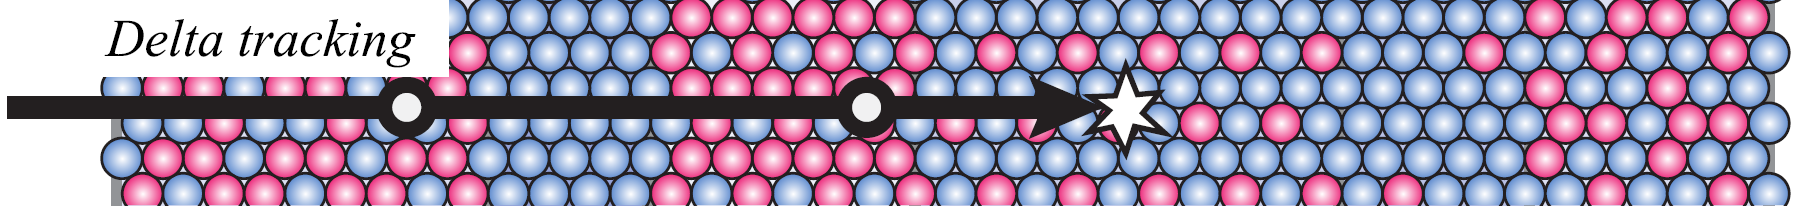
\includegraphics[width=0.8\linewidth]{img/novak_delta_tracking.png}
    \caption{For delta tracking we add fictious matter (red circles) to obtain a homogeneous medium (Image from \cite[p. 6]{novak_overview}).}
    \label{fig:novak_delta_tracking}
\end{figure}
To estimate the transmittance in a heterogeneous medium we employ a similar algorithm called \textit{ratio tracking} \cite{novak_ratio_tracking}.
As opposed to delta tracking, ratio tracking does not compare whether the interaction is a null-collision \cite[p. 4]{novak_ratio_tracking}.
Instead it updates the transmission with $T_{new} = T_{old}(1 - \frac{\mu_t(\boldsymbol{x})}{\bar{\mu_t}})$ \cite[p. 4]{novak_ratio_tracking}.

Since both algorithms use a global majorant of the extinction they perform poorly in media where the extinction varies strongly across the medium.
Therefore we use local majorants as suggested in the paper \citetitle{brick_grid} by \citeauthor{brick_grid} \cite{brick_grid}.
\begin{figure}[!ht]
    \centering
    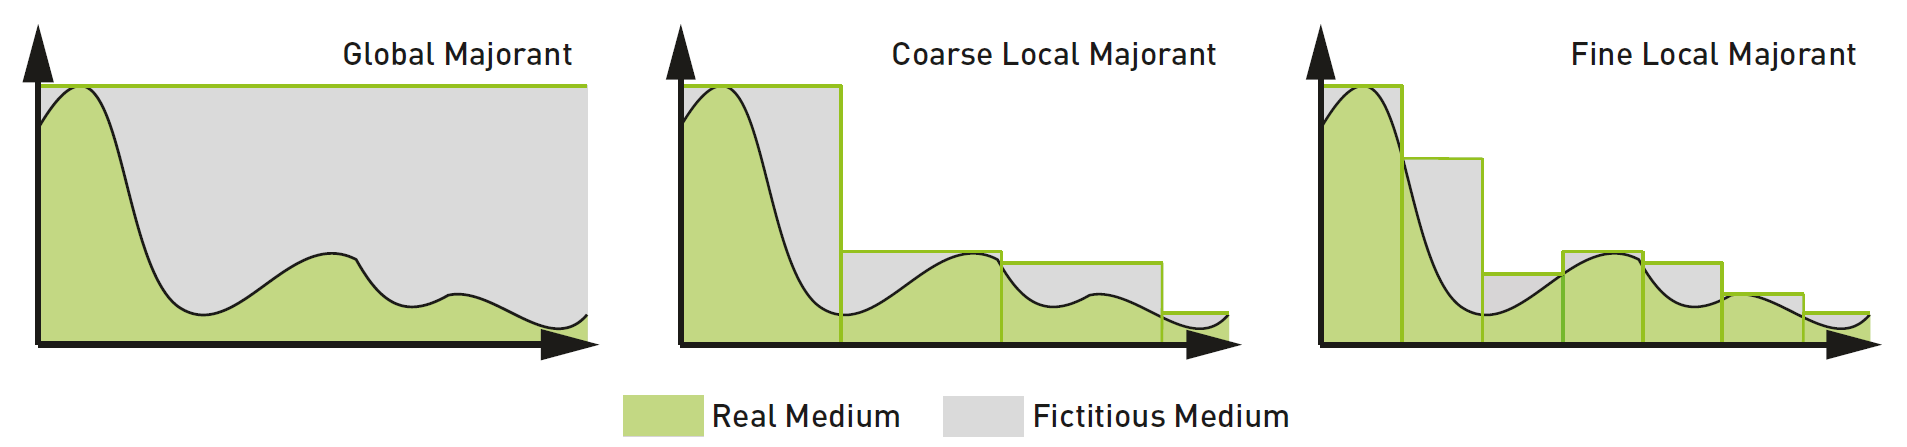
\includegraphics[width=0.9\linewidth]{img/brick_grid_majorants.png}
    \caption{Visualization of the concept of local majorants. These allow to sample distances and estimate transmittance more efficiently (Image from \cite[p. 3]{brick_grid}).}
    \label{fig:brick_grid_datastructure}
\end{figure}
To store the volume data we use three textures.
First we use an \textit{atlas texture} to store \textit{bricks} which are groups of $8 \times 8 \times 8$ voxels \cite[p. 4]{brick_grid}.
The second texture is the \textit{indirection texture} which stores offsets into the atlas.
This texture therefore links a position in space to a brick of data in the atlas \cite[p. 4]{brick_grid}.
Finally we store the minorant and majorant of each brick in the \textit{range texture} \cite[p. 4]{brick_grid}.
These are used to scale the density values in the atlas texture to the interval $[0, 1]$ \cite[p. 4]{brick_grid}.
The range texture additionally has three mipmap levels which allows to have local majorants at different scales \cite[p. 7]{brick_grid}.
\begin{figure}[!ht]
    \centering
    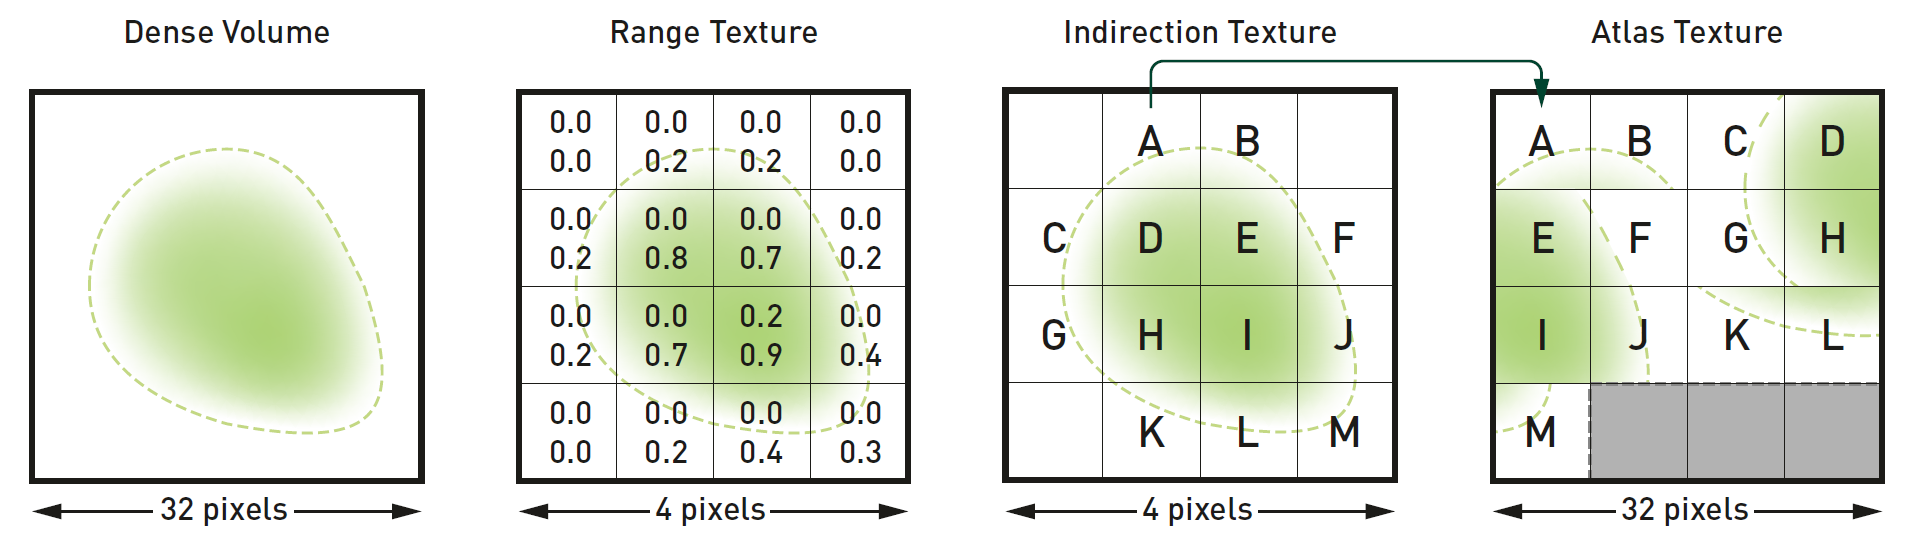
\includegraphics[width=0.9\linewidth]{img/brick_grid_datastructure.png}
    \caption{Datastructure of brick grid (Image from \cite[p. 4]{brick_grid}).}
    \label{fig:brick_grid_datastructure}
\end{figure}
Since the resulting atlas texture no longer has spatial coherence, hardware interpolation by the texture unit is not possible \cite[p. 5]{brick_grid}.
Therefore we employ a form of stochastic lookup where we jitter the lookup point by $\pm0.5$ voxels before doing point sampling \cite[p. 5]{brick_grid}.
When having a large number of lookups, as it is the case in Monte Carlo integration, this is equivalent to trilinear interpolation without introducing a significant overhead \cite[p. 5]{brick_grid}.

For distance sampling and transmittance estimation we first sample a target optical thickness $\tau_{target}=-ln(1-\xi)$ \cite[p. 6]{brick_grid}.
We then accumulate the optical thicknesses of all bricks along a ray until the accumulated thickness exceeds the target thickness \cite[p. 6]{brick_grid}.
In this case we step back along the ray until it matches $\tau_{target}$ \cite[p. 6]{brick_grid}.
Now we perform the stochastical null-collision test by comparing the density at this point with the local majorant \cite[p. 6]{brick_grid}.
In the case of distance sampling, we return the distance to the first real collision \cite[p. 6]{brick_grid}.
For transmittance estimation, we adjust the current estimate by the ratio of real to fictious matter \cite[p. 6]{brick_grid}.
When having a null-collision, the algorithm is restarted by sampling a new target optical thickness \cite[p. 6]{brick_grid}.
This is repeated until a distance is successfully sampled, the transmittance estimation is ended by russian roulette or when the ray left the volume \cite[p. 6]{brick_grid}.

\subsection{Phase functions}
\label{subsec:phase_function}
Equation \ref{eq:in_scattered_radiance} already used the term of a \textit{phase function}, now we want to explain this concept in more detail.
Similar like a \acs{brdf} gives the amount of light scattered into a certain direction on a surface, a phase function gives this amount in a volume \cite[p. 2]{novak_overview}.
The simplest phase function possible is an isotropic phase function in the form
\begin{equation}
    f_p(\omega_o, \omega_i)=\frac{1}{4\pi}.
\end{equation}
As it can be seen it has a constant value for all directions $\omega$, $\omega'$ on the unit sphere \cite[p. 2]{novak_overview}.

Since we want our \acp{lod} to look similar like the corresponding mesh representation an isotropic phase function is not sufficient.
Instead we choose the \acs{sggx} phase function \cite{sggx} because it provides scattering properties that match diffuse and specular \acsp{brdf}.
Particularly it is similar to microfacet models like the GGX \acs{brdf} \cite{ggx} which also led to the name \acf{sggx} \cite[p. 1]{sggx}.
The idea behind the GGX \ac{brdf} and other microfacet models is that a surface can be modeled by a distribution of normals which describe the roughness of the surface at a certain point \cite[p. 3]{ggx}.
Expanding on this idea \citeauthor{microflake} introduced the microflake framework which models the medium as two-sided specularly reflecting flakes which are distributed according to a certain \ac{ndf} \cite[pp. 4-5]{microflake}.
\citeauthor{sggx} define the \ac{ndf} for the SGGX phase function as:
\begin{equation}
    D(\omega_m)=\frac{1}{\pi \sqrt{|S|}(\omega_m^T S^{-1} \omega_m)^2},
\end{equation}
where $\omega_m$ is the direction of the microflake normal and $S$ is a 3 $\times$ 3 symmetric positive definite matrix which encodes the scattering properties \cite[p. 4]{sggx}.
This \ac{ndf} can be seen as the extension of the GGX \acs{ndf} to the negative hemisphere:
\begin{figure}[!ht]
    \centering
    \begin{subfigure}[b]{0.45\linewidth}
        \centering
        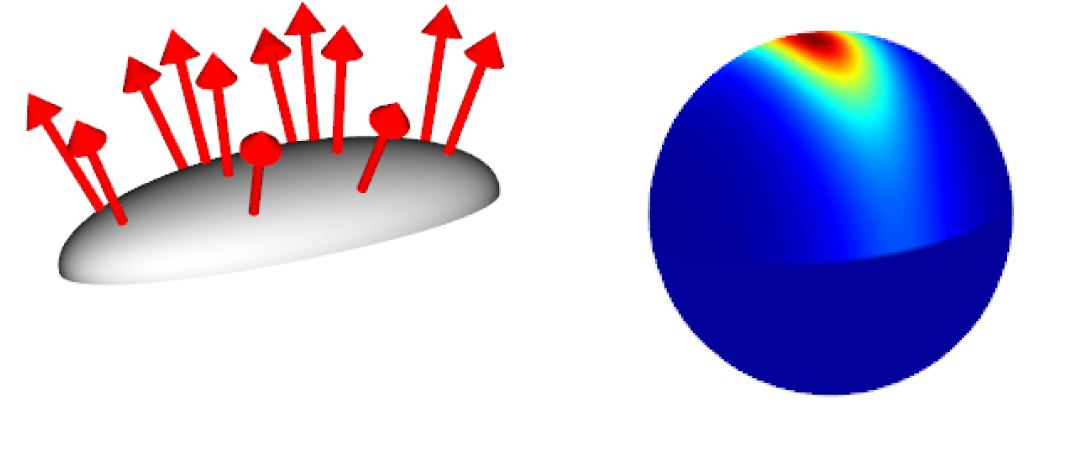
\includegraphics[width=\linewidth]{img/sggx_ndf_a.jpg}
        \caption{GGX $D(\omega_m), \omega_m \in \Omega^+$ \cite[p. 3]{sggx}}
        \label{fig:sggx_ndf_a}
    \end{subfigure}
    \begin{subfigure}[b]{0.45\linewidth}
        \centering
        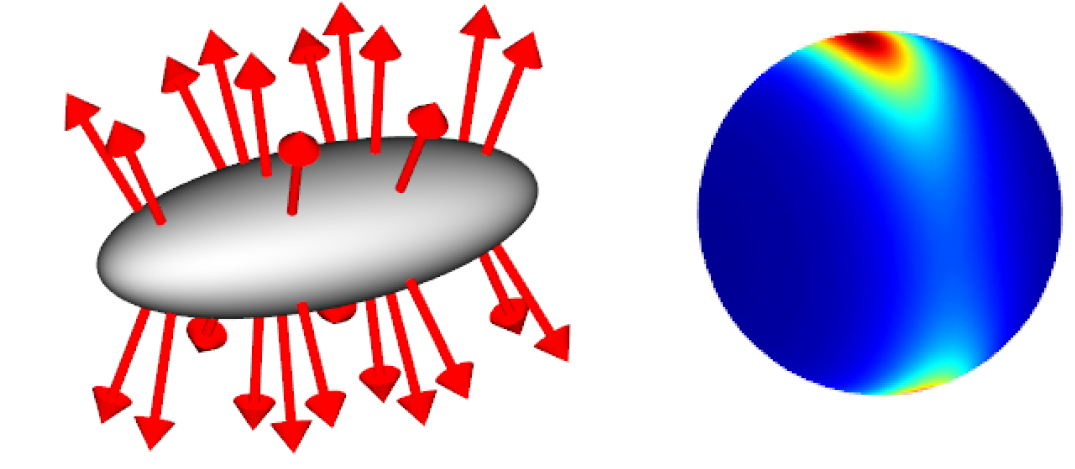
\includegraphics[width=1\linewidth]{img/sggx_ndf_b.jpg}
        \caption{SGGX $D(\omega_m), \omega_m \in \Omega$ \cite[p. 3]{sggx}}
        \label{fig:sggx_ndf_b}
    \end{subfigure}
	\caption{Visualization of anisotropic \acsp{ndf}. Note that the negative hemisphere of the SGGX \acs{ndf} is a mirroring of the positive hemisphere.}
	\label{img:sggx_ndf}
\end{figure}
Based on the \acs{ndf} the authors then introduce a \ac{vndf} $D_{\omega_o}(\omega_m)$ which is used for importance sampling of the phase function, since it reduces variance as opposed to the \acs{ndf} \cite[p. 9]{vndf_importance_sampling}.
Another important concept in the mikroflake framework is the projected area $\sigma(\omega_o)$ of the microflakes.
This is the area of the microflakes when projected onto a plane in direction $\omega_o$ \cite[p. 3]{sggx}.
\begin{figure}[!ht]
    \centering
    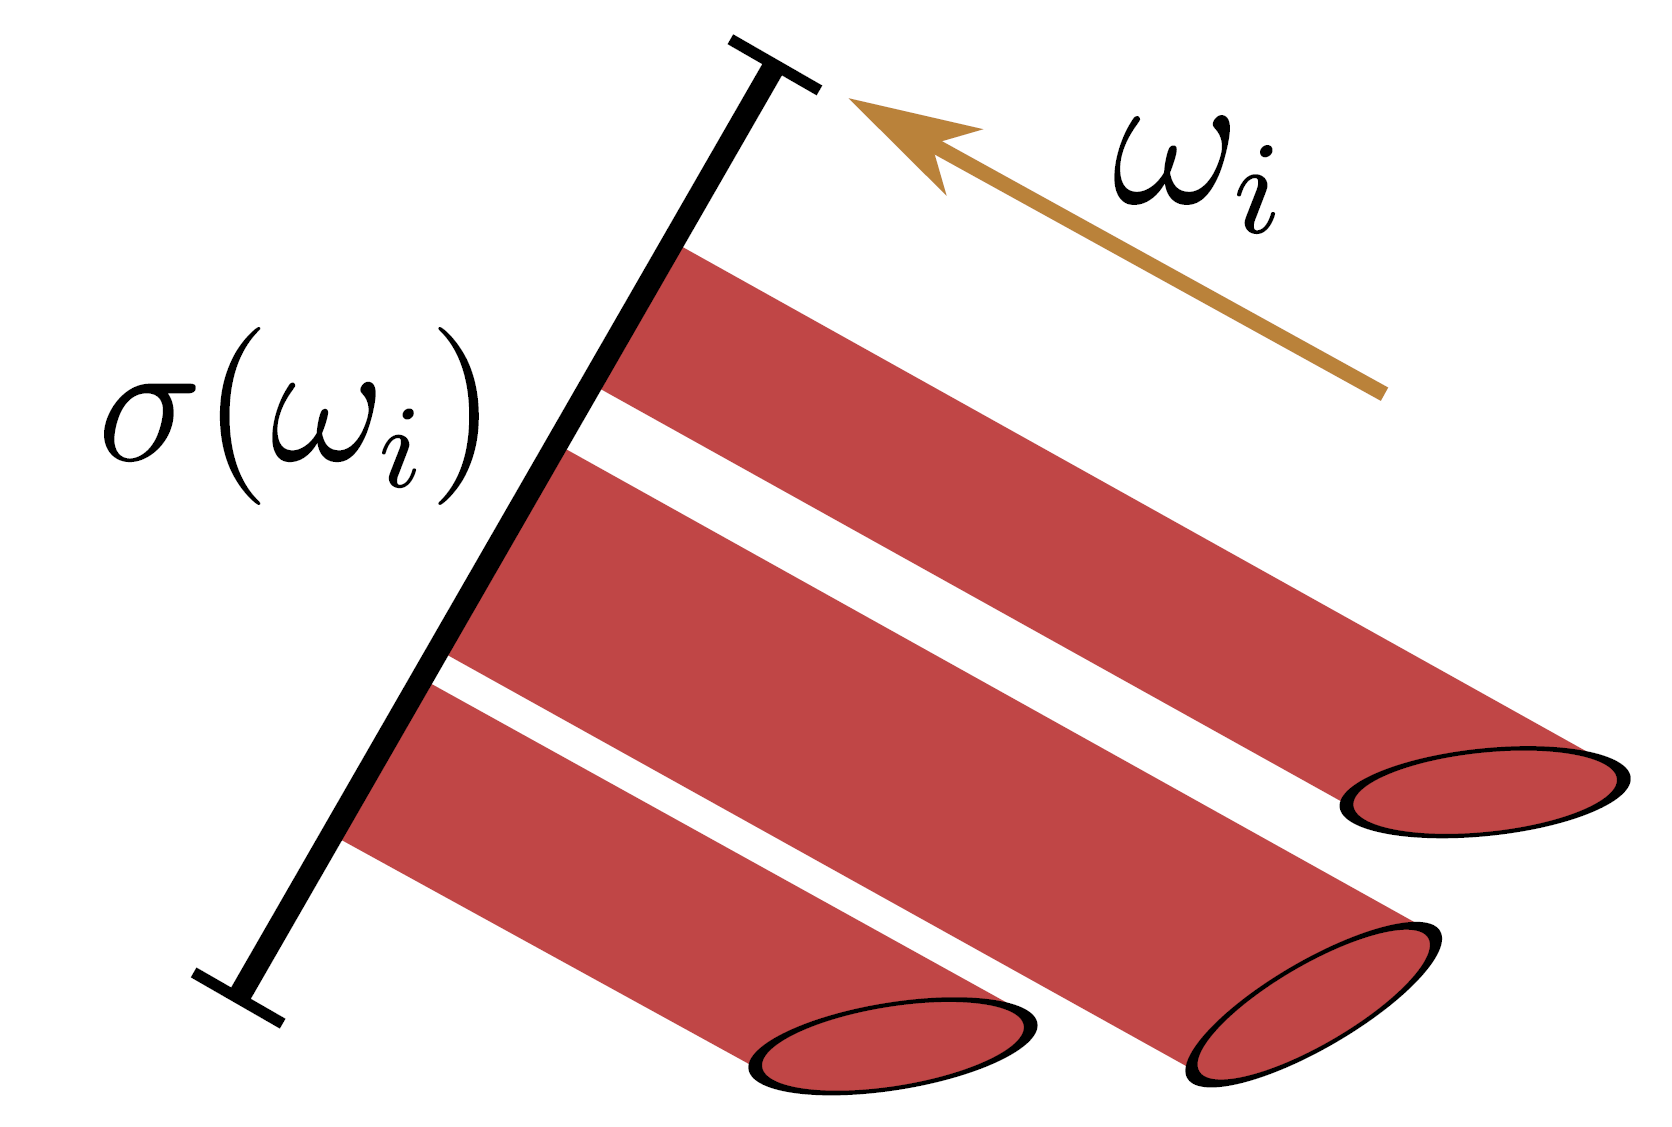
\includegraphics[width=0.3\linewidth]{img/sggx_projected_area.png}
    \caption{Projected area $\sigma(\omega_o)$ \cite[p. 2]{sggx}.}
    \label{fig:sggx_projected_area}
\end{figure}
For the SGGX phase function the projected area is defined as \cite[p. 4]{sggx}:
\begin{equation}
    \label{eq:projected_area}
    \sigma(\omega_o)=\int_\Omega \langle \omega_o, \omega_m \rangle D(\omega_m) d\omega_m = \sqrt{\omega_o^T S \omega_o},
\end{equation}
where $\langle -,-\rangle$ denotes the clamped dot product \cite[p. 3]{sggx}.
Having defined these terms the authors introduce the actual phase function which consists of a specular and a diffuse component.
The specular component is evaluated as \cite[p.7]{sggx}:
\begin{equation}
    f{}^{spec}_p(\omega_o, \omega_i) = \frac{D(\omega_h)}{4 \sigma(\omega_o)}.
\end{equation}
Importance sampling the specular component requires to sample a normal from $D_{\omega_o}$ and the direction $\omega_o$ is reflected on this normal to generate an incident direction $\omega_i$ \cite[p. 8]{sggx}.
For evaluating the diffuse phase function \citeauthor{sggx} propose to sample a normal $\omega_m$ from $D_{w_o}$ which gives an unbiased estimate of the following integral \cite[p. 8]{sggx}:
\begin{equation}
    f{}^{diff}_p(\omega_o, \omega_i) = \frac{1}{\pi}\int_\Omega \langle\omega_i,\omega_m\rangle D_{\omega_o}(\omega_m) d\omega_m = \lim \limits_{N \to +\infty} \frac{1}{N} \sum_{n=1}^N \frac{1}{\pi} \langle\omega_i,\omega_m(n)\rangle.
\end{equation}
$f{}^{diff}_p$ can then be importance sampled by generating a direction $\omega_m$ from $D_{\omega_o}$ and then sampling the hemisphere given by $\omega_m$ \cite[p. 8]{sggx}.

\section{Mesh filtering}
\label{sec:mesh_filtering}
For generating \acp{lod} we need to transform the mesh representation into volumes, we refer to this process as filtering.
We follow the approach by \citeauthor{hybrid_mesh_volume_lods} in the paper \citetitle{hybrid_mesh_volume_lods} and use ray casting to estimate the density for each voxel \cite{hybrid_mesh_volume_lods}.
To sample ray origins the authors use a \ac{pdf} $D_i=D_i^{cube} \ast D^{smooth}$ around the voxel center \cite[p. 9]{hybrid_mesh_volume_lods}.
$D_i^{cube}$ is a cubic uniform \ac{pdf} around the voxel center and $D^{smooth}$ is a 3D gaussian function with the standard deviation of 0.6 times the length of the voxel edge \cite[p. 9]{hybrid_mesh_volume_lods}.
The length of the rays is set to the length of the voxel edge \cite[p. 9]{hybrid_mesh_volume_lods}.
We deviate from this ray generation procedure as we choose the ray origin on a cubic uniform \ac{pdf} around the voxel center and clip our rays at a bounding sphere around the voxel.
Details to our procedure are explained in section \dots.
Each ray is intersected with the micro-geometry, the number of hits and the total number of rays casted determine the occlusion probability \cite[p. 8]{hybrid_mesh_volume_lods}:
\begin{equation}
    P_{occ}=\frac{nbHits}{nbRays}.
\end{equation}
Since a medium is defined on the density $\rho$ the authors solve the integral
\begin{equation}
    1 - \frac{1}{4\pi}\int_\Omega e^{-\rho\sigma_u(\omega)ray_l} d\omega = P_{occ}
\end{equation}
for $\rho$ \cite[p. 9]{hybrid_mesh_volume_lods}.
$\sigma_u(\omega)$ is the microflake projected area as defined in \ref{eq:projected_area} and $ray_l$ is again the length of the voxel edge.
This equation cannot be solved analytically and therefore requires gradient descent based optimization of $\rho$ \cite[p. 9]{hybrid_mesh_volume_lods}.
In section \dots we further explore this optimization procedure.


